\definecolor{MotorColor}{HTML}{1F77B4}
\definecolor{CueColor}{HTML}{9467BD}

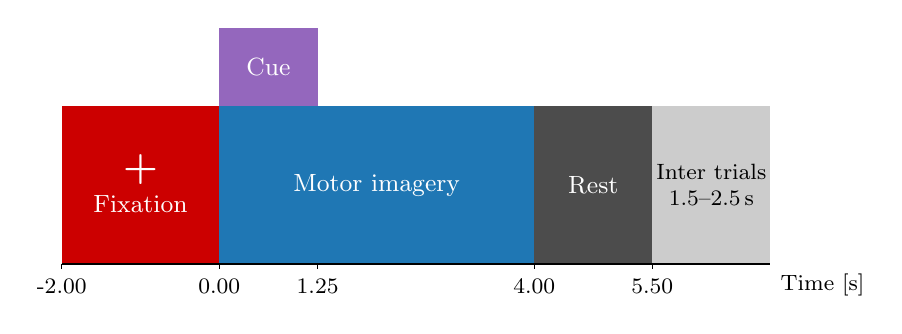
\begin{tikzpicture}

  %–– Altura de los bloques ––
  \def\boxheight{2.0}

  %–– Parámetros de la línea temporal ––
  \def\startFix{-2}
  \def\endFix{0}
  \def\endCue{1.25}
  \def\endMI{4}
  \def\endRest{5.5}
  \def\endTotal{7}

  %–– Rectángulos principales ––
  \filldraw[fill=red!80!black, draw=none] (\startFix,0) rectangle (\endFix,\boxheight);
  \filldraw[fill=MotorColor, draw=none] (\endFix,0) rectangle (\endMI,\boxheight);
  \filldraw[fill=gray!60!black, draw=none] (\endMI,0) rectangle (\endRest,\boxheight);
  \filldraw[fill=gray!40, draw=none] (\endRest,0) rectangle (\endTotal,\boxheight);

  %–– Cue encima ––
  \filldraw[fill=CueColor, draw=none] (\endFix,\boxheight) rectangle (\endCue,\boxheight+1);

  %–– Cruz y texto de fijación, ambos centrados ––
  \node[text=white,font=\Large\bfseries]
    at ({(\startFix+\endFix)/2},{0.60*\boxheight}) {+};

  \node[text=white,font=\small]
    at ({(\startFix+\endFix)/2},{0.38*\boxheight}) {Fixation};

  %–– Etiquetas de texto ––
  \node[text=white,font=\small]
    at ({(\endFix+\endMI)/2},{0.5*\boxheight}) {Motor imagery};

  \node[text=white,font=\small]
    at ({(\endMI+\endRest)/2},{0.5*\boxheight}) {Rest};

  \node[text=black,font=\footnotesize,text width=2cm,align=center]
    at ({(\endRest+\endTotal)/2},{0.5*\boxheight}) {Inter trials 1.5--2.5\,s};

  \node[text=white,font=\small]
    at ({(\endFix+\endCue)/2},{\boxheight+0.5}) {Cue};

  %–– Eje X ––
  \draw[thick] (\startFix,0) -- (\endTotal,0) node[below right,font=\footnotesize] {Time [s]};

  \foreach \x/\lbl in {
    -2/-2.00,
     0/0.00,
     1.25/1.25,
     4/4.00,
     5.5/5.50
  }{
    \draw (\x,0) -- ++(0,-2pt) node[below,font=\footnotesize] {\lbl};
  }

\end{tikzpicture}